\documentclass{article}

\usepackage{listings}
\usepackage{graphicx}
\usepackage{wrapfig}
\usepackage{float}
\graphicspath{{Images/}}

\title{Building an AI for 9-board Tic-Tac-Toe}
\author{Sam Wlody}
\date{February 10, 2017}

\begin{document}
\maketitle
\section{Standard Tic-Tac-Toe}
Tic-Tac-Toe is a two-player, zero-sum game played on a 9x9 board. Each player takes turns placing their letter, either an X or an O on the board, until they get three in a row either horizontally, vertically, or diagonally, or the board is full. An AI was implemented for this using adversarial state-space search, the specifics of which will now be discussed.
\begin{figure}[H]
	\centering
	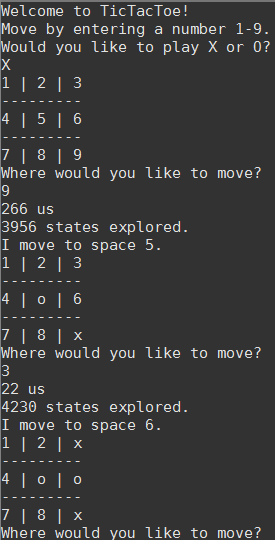
\includegraphics[width=0.4\linewidth]{TicTacToeScreen.png}\\
	A sample output from running TicTacToe.c for the first couple moves
\end{figure}
\subsection{Initial build using Java}
This project started out in Java, as it is the language that I'm most comfortable in. I started out by making an object to represent the state of the game at any given time. To represent the state, you must know who has moved in what position (what the board looks like), how many moves have been made, and whose turn it currently is. The state class is largely setters and getters for the values. The state class also contains a checkMove() function, which returns whether or not the move is legal, as well as a print function which prints out the board in an easily viewable fashion and a getWinner() method, which returns whether or not the game is over, and if so, if it has tied, or who has won. From here I went about building the tree. I didn't know about the minimax algorithm by the time I started this, so I used a FIFO queue-based depth-limited search to build a tree data structure, stopping at terminal states (those that end in a win, loss, or tie). Once I learned about minimax, it was relatively easy to implement, simply moving down the tree to terminal nodes, and return the min or max values upwards.

The performance for this method was surprisingly good, with even the first move, which has the most states to explore (549,946), taking only 107 ms on average to generate the tree, and a steady 18 ms to run minimax through the tree to decide on the best possible move. However, this method ending up using over 100 MB of memory, which would not scale to the state space of 9-board. Additionally, further experimentation revealed that the optimal move was \textit{not} always being chosen for each state, for reasons I could not determine.
\subsection{Rebuilding in C}
In order to scale my program to 9-board, I decided to rewrite my program, and in the process move to C for the dual purpose of practice for myself and increased performance for the program. I ditched the tree data structure, and instead just used the minimax algorithm to search an abstract tree using recursive calls to minimax on subsequent states of the currently explored state. A state struct was still used to represent states, with an array representing the board, a variable to keep track of the player whose move it is, and the number of moves to reach the state. I also implemented a function to generate the subsequent state for a given state given a legal move, a method to return whether or not the game is over, and if somebody won, and a method to print the board of a given state.

There are four functions in the main TicTacToe.c file. The main method continuously calls the newGame() function until the player doesn't want to play anymore. There is also a getMove() function, returns a move given the minimax value of all of the possible choices for the current state. Finally, there is the minimax function itself (in this case it is modified to be negamax with alpha-beta pruning). For statistics output, I put in a states explored counter as a global variable, and a timer around the function used to return a move.

I expected this version of the program to run much faster, in addition to having a smaller memory footprint. However, the first move took 3 seconds, over 300x longer than it took in the Java program. Further analysis revealed that for the first move, rather than generating just 500,000 states like the Java program did, 25,000,000 states were being explored by minimax. Additionally, nearly 1.5 GB of memory was being used. After about 6 hours of trying everything under the sun, I found the fix, but still don't really understand why it works. The change in code that afforded this 1200x speedup and 10000x memory reduction is shown below.

\renewcommand{\lstlistingname}{Technique}
\begin{lstlisting}[caption=This code is broken, language=Python, escapeinside={(*}{*)}]
int minimax(state, max)
   if(max)
      int bestValue = -(*$\infty$ *)
      foreach(child of state)
         bestValue = max(bestValue, minimax(child, false))
      return bestValue
   (*$\dots$*)
\end{lstlisting}

\begin{lstlisting}[caption=This code works, language=Python, escapeinside={(*}{*)}]
int minimax(state, max)
   if(max)
      int bestValue = -(*$\infty$ *)
      foreach(child of state)
         int v = minimax(child, false)
         bestValue = max(bestValue, v)
      return bestValue
   (*$\dots$*)
\end{lstlisting}\vspace{5mm}

Since the only change made was putting the minimax call outside of the max() function, there must have been some compiler issue with having a recursive function call within another function. This should do nothing other than double the stack trace, but there were other unexplained side effects to this, such as calling the minimax algorithm 50x more than necessary.

One other small change I made from the Java program was the switch from minimax to negamax. These two functions return the same value and run in the same amount of time, but negamax take up about half the lines of code of minimax.

After fixing this issue, the same number of states were generated in the C program as in the Java program, and the C program was running 4x faster (30 ms for the first move), and using 1000x less memory (136 KB). Part of this performance improvement was likely due to the lower level of abstraction in C, but the other part was the simpler implementation of the program without a tree data stucture. The best performance I was able to achieve for standard TicTacToe was when I added alphabeta pruning, which reduced the decision time for the first state to 900 $\mu$s (over 30x improvement), and reduced the numbers of states explored from 550,000 to 18,000. From here, I could move to solve 9-Board.

\begin{figure}[H]
	\centering
	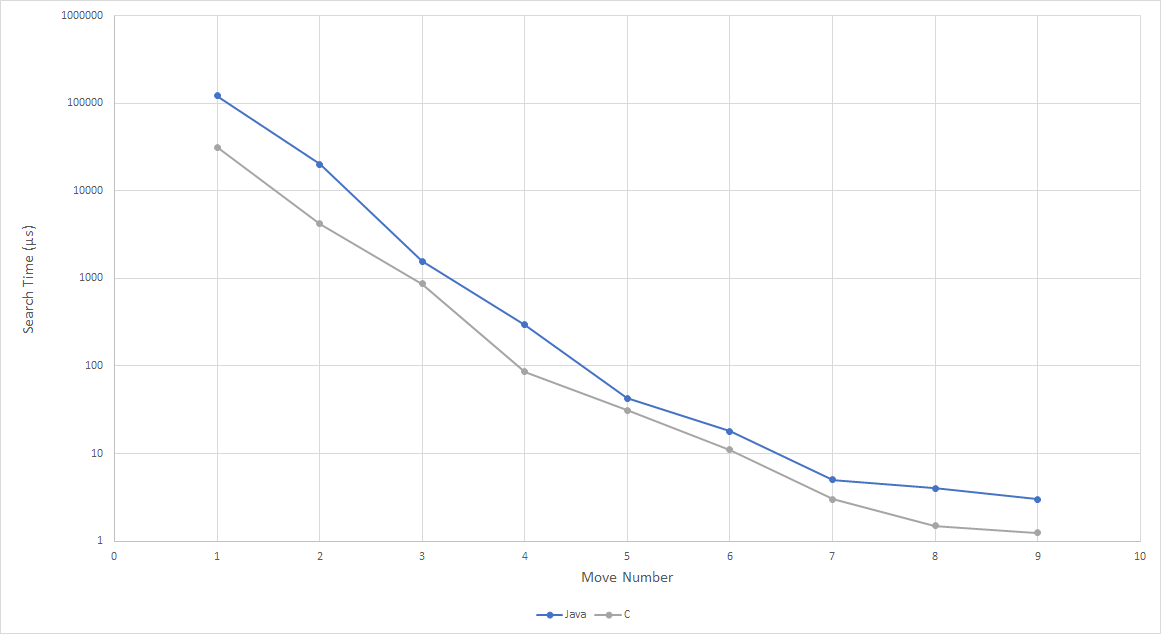
\includegraphics[width=\linewidth]{Log.png}
	On the log scale we see that C performs consistently better than Java.
	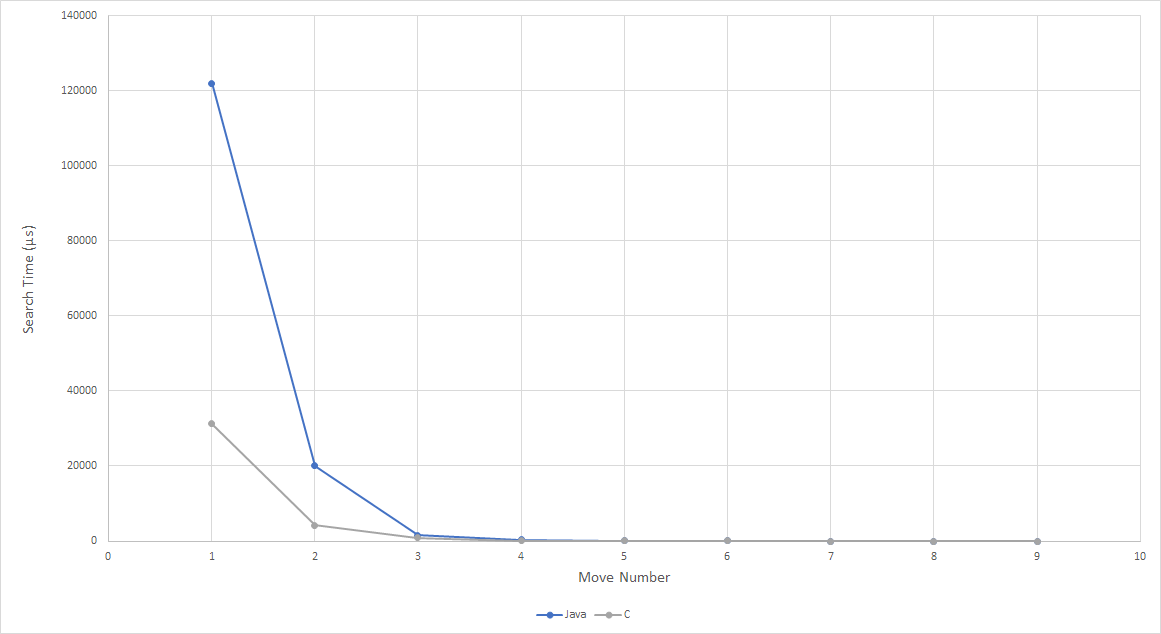
\includegraphics[width=\linewidth]{Linear.png}
	A linear scale makes it apparent how much of a difference the rewritten program makes, especially in earlier moves.
\end{figure}
\begin{figure}[H]
	\centering
	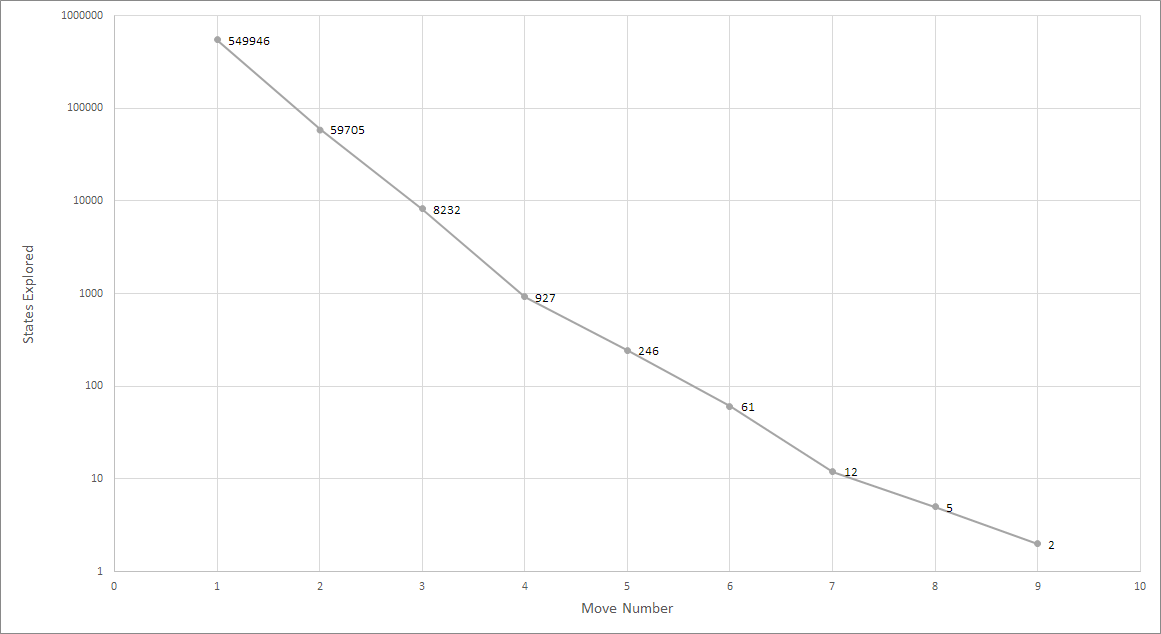
\includegraphics[width=\linewidth]{States.png}
	In both C and Java, the average number of states explored with each move number, showing a logarithmic regression as the game progresses.
\end{figure}

\section{9-board Tic-Tac-Toe}
9-board Tic-Tac-Toe has the same basic principle as regular Tic-Tac-Toe: three letters must be placed in a row for a player to win. However, 9-board is distinct in that there is a 3x3 grid of 9 boards, as the name implies. For every move within one of these boards, the other player must move in the corresponding board. For example, if X begins the game by playing in the top left board, on the bottom right square, O must respond with a move in the bottom right board. Representationally, this is not significantly different from regular Tic-Tac-Toe, however, more advanced techniques are needed to search the state space, which is prohibitively large when compared to regular Tic-Tac-Toe.

\begin{figure}[H]
	\centering
	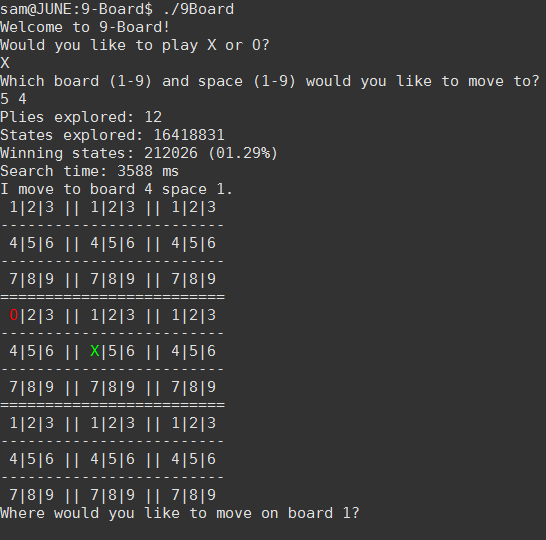
\includegraphics[width=0.75\linewidth]{9BoardScreen.png}\\
	A sample output from running 9Board.c for the first move. The computer's moves are displayed in red and the player's moves in green.
\end{figure}
\subsection{Changes from standard Tic-Tac-Toe}
In terms of representation, two arrays are needed for each state rather than just one: one 9-member array to represent the "metaboard", and for each board within that array, another 9-member array to represent each space. For example, board[0][4] (0-indexed), represents the 0th board and the 4th space, which, similarly to standard Tic-Tac-Toe, will be -1 for empty, 0 for X, and 1 for O. Wins are determined the same was as in regular Tic-Tac-Toe. For whichever board was just moved in, if there is a 3-in-a-row for either letter, the game is over, and subsequent states don't need to be explored. No possible moves for a given board results in a tie.

Aside from representation, there are three major differences between the program used for regular Tic-Tac-Toe and that used for 9-board. They are: use of Alpha-Beta pruning to reduce the number of states searched, time-limited iterative deepening to allow more states to be explored further into the game, and use of a heuristic function to estimate the value of states when an end state can not be reached by the search algorithm. All three changes stem from the fact that the search tree for 9-board is far too large to explore in a reasonable amount of time.
\subsection{Alpha-Beta pruning}
Alpha-Beta pruning is an extension of minimax which ignores states that can not achieve a better minimax score. Minimax is a recursive algorithm which traverses down the state tree, returning the value of leaf nodes up the tree. The max player, representing the computer, tries to maximize its likelihood of winning, assuming the min player, representing the player, will maximize their likelihood of winning.

Alpha-Beta pruning is an extension of this algorithm which stops searching subsequent states once it is determined that no better score can be achieved for a given state. This reduces the number of states that need to be searched, thus increasing the speed of the search.
 
I implemented it first in standard Tic-Tac-Toe, to ensure that it worked, before implementing it in 9-board. It was only a two line change to the code of negamax, which made the few issues that I encountered especially easy to debug.
\subsection{Time-limited iterative deepening}
I decided to use a time-limited iterative deepening search strategy for 9-board. Rather than using a fixed depth-limited search, using a time-limited search allows more plies to be explored further into the game. The implementation was a simple loop, which ran Alpha-Beta pruning to subsequently greater depths until a timer ran out (in this case, 1 second). Typically, the first 10-20 moves explored 10-15 ply, but once endgame approached, up to 50 moves were being explored in the allocated second.
\subsection{Heuristic function}
The heuristic function I decided on using was on that counts the total numbers of 2-in-a-rows for each player across the nine boards. Each 2-in-a-row for the computer adds 5 to the heuristic, and each one for the player subtracts 5. Wins are counted as 100 points, and ties (which I'm not sure are even possible) are counted as 0. This heuristic works decently well, but not perfectly, but if it worked perfectly it would defeat the point of using a search strategy in the first place.
\subsection{Other optimizations}
When I was first writing my program in C, I was concerned about memory requirements when I eventually moved to 9-board. I decided to use a char data type for most the numbers in the program, rather than int, as char has a size of 1 byte compared to int's 4 bytes. I am not sure how significant of an improvement this made, but in theory the program should use about half as much memory as it would if I had used int.

Another optimization I attempted to implement was ordering of the moves using the heuristic function prior to Alpha-Beta search. This should increase the number of cutoffs, and reduce the number of states that need to be explore. I found that the number of cutoffs was increased. For the first move, 2,000,000 states were explored rather than 2,020,000 - a 0.1\% difference. The program also took 4x longer to run. I suspect that this was due to the lengthy runtime of the heuristic function which is normally only called for leaf nodes, but in the case of move ordering must be called for every explored state. I did not try to change the heuristic function, but perhaps using a simpler heuristic for move ordering could improve the performance of the program.
\subsection{Issues encountered}
The majority of the issues I encountered when working on this project were caused by having to fight with C to get it to do what I wanted. One major issue I had, for example, occurred when implementing my heuristic function. Every change I made to the heuristic function resulted in the same output by the program. I spent hours trying to figure out what the problem was, stepping through each function dozens of times in GDB. Just as I was about to give up, I noticed that the function name was spelled differently in the header file (State.h) from how it was spelled in State.c. It turns out that C will not return a compilation error for an undefined function in this case, even though it cannot access the function, and the function will always return 0. The solution to this is to always compile with -Wall, which I have learned to include in all my makefiles from now on.

One other issue I had that I never ended up solving was adding randomness to the moves. I used two different methods to do this, and neither worked. The first one was to see if two moves have the same minimax value, and if so, choose one of them randomly. The second one was shuffling the moves to be explored prior to running minimax search on them. Even though the computer did not end up making the same exact moves each time the game was run, it started to lose some games. I'm still unsure about the cause for this, and did not have time to investigate it further.

The rest of the issues I encountered were trivial and don't deserve being written about here.
\section{Conclusion}
This was a fun project to work on, and I think I learned a lot about how search strategies worked and also improved my C programming quite a bit. This also ended up being the first game AI I've programmed that I could not defeat on my own. Overall I was proud with the end product both in terms of the code that I wrote being relatively minimal, and the program performing well in both speed and accuracy.
\end{document}          
